%%% Lecture Notes for Math 340
%%% Author: Stefan Eng
\documentclass{article}

\usepackage[utf8]{inputenc}
\usepackage[top=1.5in,left=1in,right=1in,bottom=1.5in,headheight=1in]{geometry}
\usepackage{fancyhdr}
\usepackage{lastpage}
\usepackage{amsmath,amsthm,amssymb}
\usepackage{graphicx}
\usepackage{theoremref}

\graphicspath{{./images/}}


% mymacros.sty
\usepackage{math340_macros}

%%%%%%%%%%%%%%%%%%%%%%%%%%%%%

\theoremstyle{plain}
\newtheorem{axiom}{Axiom}
\newtheorem{thm}{Theorem}[section]

\theoremstyle{definition}
\newtheorem{defn}{Definition}[section]
\newtheorem{exmp}{Example}[section]

\theoremstyle{remark}
\newtheorem*{note}{Note}



\renewcommand\qedsymbol{\ensuremath{\blacksquare}}
%%% Heading %%%
\pagestyle{fancy}
\rhead{Stefan Eng}
\cfoot{Page\ \thepage\ of\ \pageref{LastPage}}
%%%

\begin{document}

% Uncomment when we want title page and table of contents
%% Title page for the Math 340 class notes

\begin{titlepage}
\thispagestyle{empty}
\begin{center}
\textsc{\LARGE \bfseries Introduction to Probability}\\[.3cm]
\HRule \\[.5cm]
\textsc{\large California State University\\Northridge}\\
\HRule \\[1cm]
\textsc{\large Stefan Eng}
\vfill

{\large Fall 2013}

\end{center}
\end{titlepage}

%\tableofcontents
%\vfill
%\pagebreak

\section{Discrete Probability}

\subsection{Terms}
Some basic definitions.
\begin{defn}[Mutually Exclusive] \thlabel{excl}
Two events, A and B, are said to be \textbf{mutually exclusive} or \textbf{disjoint} given that:
$$
P(A \cap B) = \emptyset
$$
\end{defn}


\begin{defn}[Conditional Probability] \thlabel{cond}
The probability of A occurring given that B already occurred is equivalent to:
$$
P(A|B) = \frac{P(A \cap B)}{P(B)}
$$
\end{defn}

%\subsection{Set Theory}
%Some basic set theory is needed in the study of probability.

\subsection{Axioms}
E is an event. $S$ is the sample space. $E \subseteq S$. To every event in $S$ we assign a probability, $P(E)$. Then following axioms hold:
\begin{axiom} \thlabel{axiom1}
The probability of an event is a non-negative real number.
$$
P(E) \in \mathbb{R}, P(E) \geq 0
$$
\end{axiom}

\begin{axiom} \thlabel{axiom2}
Something will always happen.
$$
P(S) = 1
$$
\end{axiom}

\begin{axiom} \thlabel{axiom3}
For countable, disjoint events $E_1,E_2,\ldots$:
$$ 
P(E_1 \cup E_2 \cup \cdots) = \displaystyle \sum_{i=1}^{\infty} P(E_i)
$$
\end{axiom}

\subsection{Sample Point}
The \textit{sample point method} of calculating probability involves calculating all possible ways an event can happen and see what part of the total number of possible events this is.
%\begin{enumerate}

%\end{enumerate}
\subsubsection{Tools for Sample Point}
If we have a sample space that has $N$ points, each with equal probability of occurring, then given a event $E$ contains $n_i$ sample points, the probability of $E$ occurring is:
$$
P(E) = \frac{n_i}{N}
$$
This is the basis for how we will calculate the probability with the following ways to count sample points.

\begin{thm}[$mn$ rule] \thlabel{mn}
With $m$ elements $a_1, a_2, \ldots, a_m$ and $n$ elements $b_1, b_2, \ldots, b_n$, it is possible to form $mn = m \times n$ pairs. This is equivalent to the number of pairs in the Cartesian Product ($A \times B$).
\end{thm}

\begin{figure}[h!]
\centering
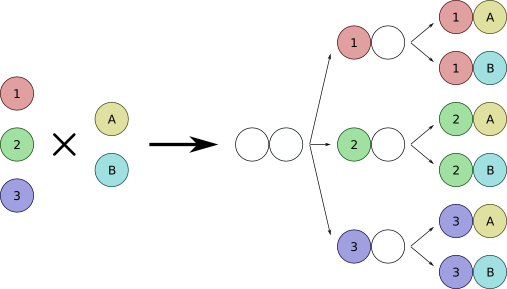
\includegraphics[scale=.5]{counting_mn}
\caption{mn rule}
\label{mn_diagram}
\end{figure}


\subsection{Event Composition}

\subsection{Bayes' Theorem}
% Uncomment for tree picture
%\begin{figure}[h!]
%\centering
%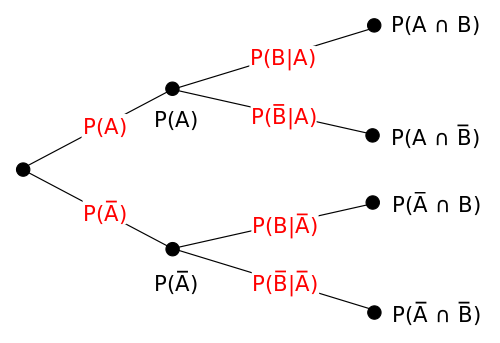
\includegraphics[scale=.5]{tree_diagram}
%\caption{Tree Diagram}
%\label{tree}
%\end{figure}

\begin{defn}[Partition] \thlabel{part}
For some positive integer $k$, let the sets $B_1,B_2,\ldots,B_k$ be such that:
\begin{enumerate}
\item $S = B_1 \cup B_2 \cup \cdots B_k$.
\item $B_i \cap B_j = \emptyset$, for $i \not = j$.
\end{enumerate}
\end{defn}

\begin{thm}[Law of Total Probability] \thlabel{totalprob}
  Assume that $\{B_1, B_2, \ldots, B_k\}$ is a partition of S (see Definition \thref{part}) such that $P(B_i) > 0$, for $i = 1, 2, \ldots,k$. Then for any event $A$.
  $$
  P(A) = \displaystyle \sum_{i=1}^k P(A|B_i) P(B_i)
  $$
  or, alternatively,
  $$
  P(A) = \displaystyle \sum_{i=1}^k P(A \cap B_i)
  $$
\end{thm}
\begin{proof}
  Assume A is a subset of S. Then we can write A as:
  \begin{align*}
    A &= A \cap S\\
      &= A \cap (B_1 \cup B_2 \cup \cdots \cup B_k)\\
      &= (A \cap B_1) \cup (A \cap B_2) \cup \cdots \cup (A \cap B_k)
  \end{align*}
  Since $\{B_1, B_2, \ldots, B_k\}$ is a partition of S, if $i \not = j$,
  \begin{align*}
    (A \cap B_i) \cap (A \cap B_j) &= A \cap (B_i \cap B_j)\\
    &= A \cap \emptyset\\
    &= \emptyset
  \end{align*}
  Thus, $(A \cap B_1)$ and $(A \cap B_j)$ are mutually exclusive events (see \thref{excl}). It follows that,
  \begin{align*}
    P(A) &= P(A \cap B_1) + P(A \cap B_2) + \cdots + P(A \cap B_k)\\
    &= P(A|B_1)P(B_1) + P(A|B_2)P(B_2) + \cdots + P(A|B_k)P(B_k)\\
    &= \displaystyle \sum_{i=1}^k P(A|B_i)P(B_i)
  \end{align*}
\end{proof}

\begin{note}
The Law of Total Probability is used when $P(A|B_i)$ is easier to calculate then $P(A)$.
\end{note}

\begin{thm}[Bayes' Theorem] \thlabel{bayes}
Assume that $\{B_1,B_2,\ldots,B_k\}$ is a \textbf{partition} of S (see \thref{part}) such that $P(B_i) > 0$, for $i = 1,2,\ldots,k$. Then
$$
P(B_i|A) = \frac{P(A|B_j)P(B_j)}{\displaystyle \sum_{i = 1}^k P(A|B_i)P(B_i)}
$$
\end{thm}
\begin{proof}
The proof follows from the definition of conditional probability (see \thref{cond}) and the law of total probability (see \thref{totalprob}).
$$
P(B_j|A) = \frac{B(A \cap B_j)}{P(A)}
$$
\end{proof}
\end{document}

%%% End assignment %%%

